\chapter{The Requirements Specification}
\graphicspath{ {./chapter03/Fig} }

Specification • (n) A detailed and exact statement of particulars, a
statement fully describing something to be built.---American Heritage
Dictionary

The Requirements Specification identifies those requirements that the
design must satisfy in order for it to be successful. It is in effect
the mission statement that drives all subsequent stages of development,
and when completed should be a detailed and complete vision of the
design goals. An effective Requirements Specification should identify
all important requirements, yet provide enough flexibility for the
design team to develop innovative solutions. It also serves as a
communication tool for everyone involved in the design, such as
engineering, marketing, and the client. All parties should agree to the
requirements before further development proceeds. In some cases, the
Requirements Specification serves as a legally binding agreement between
the developers and the client.

A major challenge in developing the requirements is in many ways
analogous to the proverbial ``\emph{What came first, the chicken or the
egg?}'' question. The final solution is analogous to the chicken and the
requirements are analogous to the egg. In the beginning, the chicken is
hidden inside the egg, yet the egg must be capable of describing what
the chicken will become. The difficulty is that it is hard to develop
the \emph{what} for the requirement without already having solved the
problem or created the chicken.

This chapter guides the reader through the process of developing a
Requirements Specification and is organized as follows. First, the
properties of an engineering requirement are defined and numerous
examples for computer and electrical systems are provided. Then, the
properties of the complete Requirements Specification (the collection of
marketing and engineering requirements) are considered followed by a
number of case study examples. The chapter concludes with advanced
methods of analyzing and refining requirements, utilizing tools such as
the House of Quality.

Learning Objectives

By the end of this chapter, the reader should:

\begin{itemize}
\item
  Understand the properties of an engineering requirement and know how
  to develop well-formed requirements that meet the properties.
\item
  Be familiar with engineering requirements that are commonly specified
  in electrical and computer systems.
\item
  Understand the properties of the complete Requirements Specification,
  as well as know the steps to developing one.
\item
  Be able to conduct advanced requirements analysis to identify design
  tradeoffs.
\end{itemize}

\section{Overview of the Requirements Setting Process}
\label{section':overview-of-the-requirements-setting-process}

The \emph{\textbf{Requirements Specification}}, which is the focus of
this chapter, is a collection of engineering and marketing requirements
that a system must satisfy in order for it to meet the needs of the
customer or end-user. Figure 3.1 illustrates a process for developing a
Requirements Specification that is from the \ul{IEEE Guide for
Developing System Requirements Specifications} {[}IEEE Std.
1233-1998{]}. This process is the focus of this chapter and there are
three stakeholder groups in it -- the customer, the environment, and the
technical community. The input from the customer includes the marketing
(raw) requirements that were addressed in Chapter 2. The environment
introduces requirements in the form of constraints and standards that
impact or limit the design. The input from the technical community is
based upon the knowledge of engineers who are primarily responsible for
design, implementation, testing, manufacturing, and maintenance of the
system.

\begin{figure}
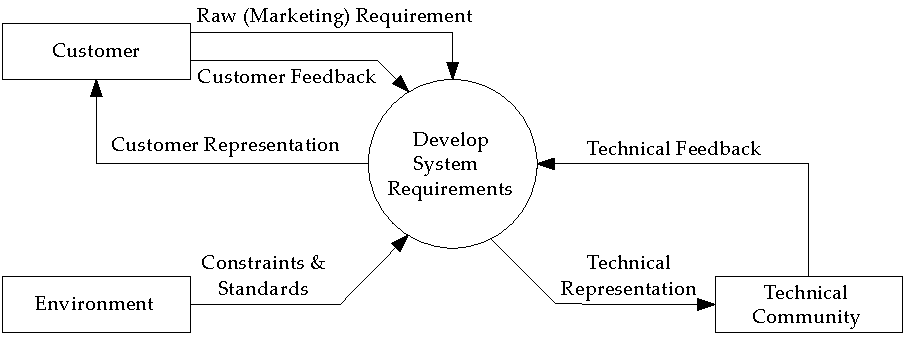
\includegraphics[width=4.6in,height=1.7in]{image1.pdf}
\caption{Requirements Specification development processes
from IEEE Std. 1233-1998. The three input sources to the process are the
customer, environment, and technical community.}
\label{figure: }
\end{figure}

\section{Engineering Requirements}
\label{section:engineering-requirements}

Before developing the complete Requirements Specification, designers
need to first determine individual engineering requirements.
\emph{\textbf{Engineering requirements}} are short statements that
address a technical need of the design. A simple example is ``\emph{The
system should be able to supply 50 watts of power.}'' This section
identifies the desirable properties of engineering requirements, methods
of identifying requirements, and provides numerous examples.

\subsection{Properties of an Engineering Requirement}
\label{section:properties-of-an-engineering-requirement}

Each engineering requirement should meet the four properties below
{[}IEEE Std. 1233-1998{]}:

\begin{enumerate}
\def\labelenumi{\arabic{enumi})}
\item
  \emph{Abstract.} This means that a given requirement should specify
  \emph{what} the system will do, not \emph{how} it will be implemented.
  This is the chicken and egg problem described earlier. It is
  frequently the most difficult property to satisfy since designers
  often have a preconceived concept for the solution. Unless absolutely
  necessary, the requirements should say nothing about the
  implementation. For example, a requirement stating that a certain
  microcontroller (i.e., technology) \ul{will} be used should be
  avoided. Admittedly, this is not always possible due to customer
  constraints or in cases where a system is being built upon
  pre-existing technology. A common analogy used for the ``\emph{what
  versus how}'' problem is that of designing a bridge. The requirement
  is to transport people from one side to other, without specifically
  stating the solution is a bridge, because another solution, like a
  ferry, may be a much more effective solution.
\item
  \emph{Verifiable.} Verifiability means that there should be a way to
  measure or demonstrate that the requirement is met in the final system
  realization. Doing so allows the system to be tested or verified
  against the requirements. The idea is that if there is no way to
  verify that the requirement is met, then it should not be a
  requirement. Verifiability is used to answer the question of
  ``\emph{Are we building the system correctly?}''
\item
  \emph{Unambiguous.} Each requirement should have a single unambiguous
  meaning and be stated with short complete sentences.
\item
  \emph{Traceable.} Requirements should be traceable marketing
  requirements. If the design doesn't satisfy the customer's needs, it
  won't be successful.
\end{enumerate}

Let's examine an example requirement for a robot whose objective is to
navigate autonomously within a specified environment. Consider the
following requirement

\begin{quote}
The robot must have an average forward speed of 0.5 feet/sec, a top
speed of at least one foot/sec, and the ability to accelerate from
standstill to the average speed in under one second.
\end{quote}

Are the four properties for an engineering requirement met? In terms of
the abstractness property, the answer is yes; it states what the system
must do, not how it will be implemented. In terms of the second
property, can the requirement be verified? Speed and acceleration are
directly testable in the final realization, and thus it is verifiable.
Is it unambiguous? It gives clear bounds for speed and acceleration.
Finally, traceability can't be shown without the marketing requirements
and is addressed later.

Now we analyze a second example requirement for the robot to see if it
meets the properties

\begin{quote}
The robot must employ IR sensors to sense its external environment and
navigate autonomously with a battery life of one hour.
\end{quote}

This requirement is not abstract since it identifies part of the
solution in terms of the sensor type and the fact that batteries must be
used. It is somewhat ambiguous in that it should specify what is meant
in terms of autonomous and the operating period. In terms of operating
period, should it work for exactly one hour and stop, or is greater than
an hour acceptable? Again, traceability can't be demonstrated without
the marketing requirements. This requirement would be hard to verify
without a good definition of what autonomous navigation in this context
means. A better requirement would be

\begin{quote}
The robot must navigate autonomously, with the aid of only landmarks in
the specified environment, for a period of least one hour.

Realize that good requirements typically have two key elements in the
statement -- a description capability and condition. Capability
describes what the system must do and in the above requirement, that
capability is autonomous navigation. Conditions are measurable or
testable attributes of the capability and are critical for verification.
\end{quote}

\subsection{A Fifth Property -- Realism}
\label{section:a-fifth-property-realism}

In addition to meeting the four properties, requirements should be
realistic or justified. This is not defined in the IEEE standard as a
property, but it is an important aspect that is often overlooked. To be
realistic, there should be a way of demonstrating that the target is
technically feasible. For example, a requirement could indicate that a
robot to should travel at a speed of 1,000,000 miles per hour, which
could be verifiable, unambiguous, and abstract -- yet, completely
unachievable. Realistic targets can be determined with a little
research, engineering know-how, creativity, or system modeling. One way
to do this is to assume a solution for the final system -- violating the
abstractness property. For example, consider the design of a robot where
some basic assumptions are made on the weight of the robot, the motors
used, the wheel size, and the battery selected. An engineering model
based upon these characteristics could be developed to predict
performance and estimate realistic requirements. Alternatively, target
requirements can be based upon an actual prototype, where a model or
experimental system is developed to show that a particular requirement
is feasible. This is how the technical community in Figure 3.1 feeds
into the requirements process.

The use of benchmarking to identify similar systems and their
performance provides a reference for realistic targets. It is generally
hard to surpass the performance of well-developed products and systems
on a first-generation design. An exception is with new and innovative
approaches that allow you to surpass the competition. Competitive
benchmarks may also be obtained from similar, but not necessarily
identical, products. Experience working with a particular technology or
previous generations of a system also provides guidance in selecting
realistic targets. That being said, organizations wishing to gain or
maintain a market edge often press the development team to achieve
performance on new generations that were once believed to be
unrealistic. Sometimes it just may not be feasible to determine the
technical feasibility of requirements. In such cases, the requirements
should have a certain amount of tolerance built into them and be updated
as development proceeds.

\subsection{Constraints}
\label{section:constraints}

One of the inputs to the requirements process in Figure 3.1 is the
environment, serving as the source of both constraints and standards. In
reality, all engineering requirements impose some sort of constraint on
a design, but in design a constraint is a special type of requirement. A
\emph{\textbf{constraint}} is a design decision imposed by the
environment or a stakeholder that impacts or limits the design.
Constraint requirements often violate the abstractness property. For
example, a constraint requirement is

\begin{quote}
\emph{The system must use a PIC18F52 microcontroller to implement
processing functions.}
\end{quote}

This constraint requirement specifies how the system will be
implemented. This could be because the project sponsor has developed a
great deal of expertise using this particular microcontroller and does
not want to spend the development time learning a new platform. Note
that a number of other references define constraints to be synonymous
with non-functional requirements (usually indicated as items that are
not specifically functions). However, that terminology is avoided here
since it is not well defined nor universally accepted.

\subsection{Standards}
\label{section:standards}

\emph{\textbf{Standards}} are exactly what the name implies, a standard
or established way of doing things that ensure interoperability. Without
standards, the use of technology would be severely limited, if not
downright impossible. Standards ensure that products work together, from
home plumbing fixtures to the modules in a modern computer. Imagine if
every computer manufacturer had their own communication standard,
instead of following established protocols such as RS-232, TCP/IP, and
USB---computers would have a hard time printing, sending email, instant
messaging, or surfing the Internet! Furthermore, standards ensure the
health and safety of products that people use every day. Identifying and
following standards is an expected part of good engineering practice.

The focus in this chapter is on identifying standards that impact the
requirements and ultimately the design. The question becomes, what
standards are relevant to your project and how do you use them? There
are different levels of interaction with standards that we denote as:
user, implementation, and development levels. At the \emph{user level},
the standards are simply employed in the design, and detailed technical
knowledge of the standard is typically not necessary. For example, when
using a component that communicates to other devices, it is likely that
a standard communication protocol is used. Other than having to
configure software or hardware to communicate with the standard,
detailed knowledge of the standard isn't required. Another example would
be in developing software to display digital images in a standardized
format such as JPEG-2000 (Joint Photo Experts Group), in which case it
is likely that existing software components would be used to read and
display data in this format.

At the \emph{implementation level} details of the standard need to be
understood. Standards at the implementation level are most likely to
impact the design and the requirements. For example, when developing
low-level drivers for computer peripherals, you need to become an expert
on the underlying standard. Another example is reliability, where the
requirement may be that ``\emph{the system will have a reliability of
95\% in 10 years.}'' In this case a reliability standard, such as
\ul{Military Handbook for Reliability Prediction of Equipment}
{[}MIL-HDBK 217F{]} may be employed, and its usage requires an
understanding of both the reliability theory and the standard itself.

New standards are constantly being developed and existing ones modified,
leading to the final level of interaction at the \emph{development
level}. Depending upon the standard, engineers from different
organizations, professional societies, and corporations take part in the
standards setting process. Many participants in this process are trying
to gain a competitive advantage for their products and services.

It can be difficult to navigate the world of standards; they tend to be
highly detailed and limited parts of a standard may apply to a project.
In addition, many standards are costly to obtain, while some are freely
distributed. The following is advice for identifying and employing
standards. First, conduct research on applicable standards. Virtually
all standards organizations maintain websites that provide basic
information on their particular standards. The IEEE Xplore database is a
good place to start since it has a wide variety of standards and
provides free searchable abstracts. Many companies and universities have
subscriptions databases of complete standards. Second, determine the
expected level of interaction. Based upon your analysis of the problem,
do you foresee applying standards? Or will you need to develop an
in-depth knowledge at the implementation level? In the latter case, you
need to obtain detailed information on the applicable standards.
Finally, you should consider asking your client. They may have their own
internal standards and procedures to follow, and they may have experts
on the applicable standards.

The list below identifies some of the types of standards that may be
employed in a project and included in the requirements.

\begin{itemize}
\item
  \emph{Safety}. Safety standards address how to design for safety and
  how to test products to ensure that they are safe.
\item
  \emph{Testing}. Testing standards are often related to safety, but are
  broader in scope. For example, standardized benchmark tests are used
  for comparing computational performance, one well-known standard being
  the SPEC (Standard Performance Evaluation Corporation) benchmarks.
\item
  \emph{Reliability}. Reliability standards address general reliability
  principles and design methods for different classes of systems.
  Another practical aspect is in the estimation of reliability of
  electronic systems, such as the IEEE and military reliability
  standards.
\item
  \emph{Communications.} They address how electronic systems communicate
  and transfer information, such as in computing, telephony, and
  satellite communications.
\item
  \emph{Data Formats}. Standard data formats ensure that systems and
  software can properly share information. Examples include image,
  video, and database standards.
\item
  \emph{Documentation}. There are standards for technical report
  documentation. In addition, there are standards for documenting
  processes and business practices, a well-known case being the ISO
  (International Standards Organization) 9000 and subsequent standards.
\item
  \emph{Design Methods.} Certain design techniques are standardized as
  well. Examples include software design methodologies, and the use of
  design languages such as the Hardware Description Language (HDL) and
  the Unified Modeling Language (UML).
\item
  \emph{Programming Languages.} Programming language syntax is
  standardized so that software maintains a level of portability between
  systems and compilers.
\item
  \emph{Connector Standards.} Standards for cable connections are common
  and should be followed to ensure that systems are easily interfaced
  and manufactured.
\item
  \emph{Meta-Standards.} Some standards are a combination of multiple
  standards known as meta-standards. For example, the RS-232 standard is
  really a combination of a mechanical standard describing the connector
  physical dimensions connector, an electrical standard describing the
  voltages, a functional standard describing the pins and their
  function, and a procedural standard describing how entities
  communicate.
\end{itemize}

\subsection{Identifying Engineering Requirements}
\label{section:identifying-engineering-requirements}

There are many techniques for identifying requirements listed below
{[}IEEE Std. 1233-1998{]}:

\begin{itemize}
\item
  Structured workshops and brainstorming sessions.
\item
  Interviews, surveys, and questionnaires.
\item
  Observation of processes or devices in use.
\item
  Competitive benchmarking and market analysis.
\item
  Prototyping and simulations.
\item
  Research and technical documentation review.
\end{itemize}

Many requirements may be specified for a design, but knowing which to
include is the challenge. The remainder of this section is a guide to
describe the types of engineering requirements that may be specified for
electrical and computer systems. Requirements in categories of
performance and functionality are presented first as they are often
critical, followed by an alphabetical grouping of a potpourri of other
types requirements. \textbf{This taxonomy of requirements is by no means
definitive or inclusive of all possibilities, and the design team needs
to carefully determine those that are applicable to the particular
situation. Careful attention must be given to the verifiability of
requirements for the particular application.}

\subsection*{Performance}
\label{section:performance}
\addcontentsline{toc}{subsubsection}{Performance}

These requirements reflect a critical aspect of the performance of the
system or device. They often are characterized by time, accuracy,
throughput, or percentage error. The following is an example requirement
that might be used in a security application with camera surveillance.

\begin{quote}
\emph{The system should detect 90\% of all human faces in an image.}
\end{quote}

In order to verify this, a test might be constructed where the system is
presented with a large database of face images that the system was not
developed or trained with. The number of faces correctly detected would
then be determined. Here is another example performance requirement for
a system that measure part location

\begin{quote}
The system should be able to measure part location to within ± 1mm.
\end{quote}

One way to verify this would be to take independent measurements of the
system's ability to measure part location and compare them to the result
of the system. The following is an example that could apply to software
response time.

\begin{quote}
The system should retrieve the user data no less than three seconds for
90\% of requests and in a maximum of six seconds for all requests.

This could be verified by constructing a test where a large number of
queries for user data are presented to the software under a variety of
operating conditions and the response time measured. Yet another example
is

The system should be able to process video data at a rate of 30 frames
per second.

This could be verified by providing an input video stream at the frame
rate and testing to ensure that proper processing occurs. The test
procedure would need to specify length and number of videos to test,
issues that are addressed in Chapter 7. A final example of performance
is one that could apply to electrical audio amplification

The amplifier will have total harmonic distortion of less than 1\%.

Total harmonic distortion is a measure that quantifies how closely an
amplifier is able to replicate the original signal. This would likely be
verified using laboratory instrumentation to measure the harmonic
distortion in the output signal.
\end{quote}

\subsection*{Functionality}
\label{section:functionality}
\addcontentsline{toc}{subsubsection}{Functionality}

These requirements describe the type of functions that a system should
perform. Often, they provide inputs, outputs, and the transformation
that the system will perform on the inputs. This is examined further in
Chapter 5, which presents functional design techniques. The following is
an example, where the input is ambient air temperature is converted to a
digital readout. It also has a performance aspect in that the accuracy
is specified.

\begin{quote}
The system will convert ambient temperature to a digital readout of
temperature with an accuracy of 1\% over the measurement range.

The following is an example from a real capstone project to develop a
wireless mouse that is worn by the user and integrated into a glove.

The system will implement the left and right button functions of a
standard mouse.

The following are several functional examples for software systems.

The user shall be able to search all five company internal databases.

The system will protect the user's identity with 128-bit encryption.

Note that in these last two cases, verification would be by inspection.
\end{quote}

\subsection*{Economic}
\label{section:economic}
\addcontentsline{toc}{subsubsection}{Economic}

Economic requirements include the costs associated with the development
(design, production, maintenance) and sale of a system. They may also
include the economic impact of the final system, such as how it will to
contribute to profits or save the user money. Two example economic
requirements are below.

\begin{quote}
The costs for developing the system (labor and parts) should not exceed
\$50,000.

The total parts and manufacturing costs cannot exceed \$500 per unit.
\end{quote}

\subsection*{Energy}
\label{section:energy}
\addcontentsline{toc}{subsubsection}{Energy}

Virtually all systems consume and/or produce energy and thus have energy
requirements. Energy consumption is the amount of power that a system
consumes, and may be specified in terms of maximum, minimum, or average
values. Example requirements are

\begin{quote}
The system will have an average power consumption of 500mW.

The system will have a peak current draw of 1A.

These requirements could be verified by measuring current and voltage
draws under the different operating conditions, or by estimating the
power drawn by all components in the system.
\end{quote}

Operating lifetime addresses how long the system will operate from a
given power source. For battery-powered devices, operating time is
critical, and the lifetime for a given source may be an important
requirement. An example of such a requirement is

\begin{quote}
The system will operate for a minimum of three hours without needing to
be recharged.
\end{quote}

Source characteristics refer to the characteristics of the input and/or
output sources, such as voltage, current, impedance, frequency, number
of phases, and power requirements. An example requirement is

\begin{quote}
The system will operate from a 12V source that supplies a maximum
current of 300mA.
\end{quote}

\subsection*{Environmental}
\label{section:environmental}
\addcontentsline{toc}{subsubsection}{Environmental}

These requirements address the impact of the design on the external
environment and usage of the earth's resources. For example, energy
usage is an important factor and example requirement is as follows

\begin{quote}
The system will use 20\% less energy than the industry average for
similar products and qualify for US Energy Star certification.

Recyclability is the ability to dismantle a product into its constituent
materials for reuse in other products. European countries have
regulations on the recyclability of consumer products. In many cases,
the producer of a product is responsible for its safe disposal once its
service life is over. An example requirement is as follows

50\% of the modular components will be able to be repaired and re-used
in similar products.
\end{quote}

\subsection*{Health and Safety}
\label{section:health-and-safety}
\addcontentsline{toc}{subsubsection}{Health and Safety}

The health and safety of anyone affected by the final product is an
especially important consideration. For example, IEEE and ANSI standards
provide guidance on safe levels for exposure to radio frequency electric
fields.

\begin{quote}
\emph{The system will not expose humans to unhealthy levels of
electromagnetic radiation and will meet conditions for safe operation
identified in ANSI Std. C95.1.}
\end{quote}

There is a tendency to think that physical harm is not an issue in
electrical and computer systems, but many electronic systems control
mechanically moving parts. Consider the design of an automatic garage
door system. An example constraint could be that

\begin{quote}
The door should stop moving if a person or object is detected in the
door path.
\end{quote}

This could also translate into further engineering requirements on the
amount of force on the door required to trigger it to stop. There are
many safety standards, and two that are widely applied for consumer
products are the UL (Underwriters Laboratory) and CE (Common European)
standards. Examples are

\begin{quote}
The system will use only UL approved components.

The final system will be meet UL and CE standards and be tested at an
independent laboratory for approval.
\end{quote}

\subsection*{Legal}
\label{section:legal}
\addcontentsline{toc}{subsubsection}{Legal}

Designs should not infringe upon existing patents, copyrights, and
trademarks, particularly if the intention is to sell the product. Patent
searches should be conducted, and search capabilities are available at
the United States Patent Office website
(\href{http://www.uspto.gov}{www.uspto.gov}). An example is

\begin{quote}
An intellectual property search will be conducted to ensure that there
is no infringement on prior patents.

This could be verified by having an external firm will conduct the
patent search and evaluate the design against existing intellectual
property.
\end{quote}

Security and privacy constraints apply to systems that handle sensitive
data or personal communications. The ability of computing systems to
withstand malicious attacks by hackers is another consideration, and the
use of firewalls or other protective measures may be warranted. Examples
are

\begin{quote}
The system will protect the user's identity with 128-bit encryption as
required by law.
\end{quote}

\subsection*{Maintainability}
\label{section:maintainability}
\addcontentsline{toc}{subsubsection}{Maintainability}

The maintenance of the system being developed and compatibility with
other systems are often considerations. Will the system be designed so
that it can be reused in future applications? This is common in software
development where the objective is to design modules that are reliable
and flexible enough to be used in other applications. It is also a
consideration in terms of the reusability of electronic or digital
components in future system upgrades. An example reuse constraint is

\begin{quote}
The software should maintain downward capability and be able to use
version 2 object libraries.
\end{quote}

After a product goes into service, it enters the maintenance phase,
where it is maintained and upgraded. In software designs this is an
important consideration, as software is regularly upgraded and
maintained. On the hardware side, maintenance can be facilitated by the
use of plug-in modules that are easily removed and replaced. Examples
are

\begin{quote}
The system will initially be available to 100 users at five field
locations, and within one year must be expanded to address usage by
5,000 users company-wide.

The system should have a modular design such that failed components can
be replaced by a technician in under 15 minutes.
\end{quote}

There may be internal restrictions on system development imposed by the
company based on their internal expertise and ability to maintain the
system, such as the following constraint requirement.

\begin{quote}
The system will use only PIC microcontrollers.
\end{quote}

\subsubsection*{Manufacturability}\label{manufacturability}
\addcontentsline{toc}{subsubsection}{Manufacturability}

A prevalent product development paradigm that used to be employed in
many engineering organizations was to ``\emph{throw the design over the
wall}.'' What this meant is that the design and development team would
create a new product and hand it off to the manufacturing team to
produce (throw it over the wall and run), often without having
considered the manufacturability of the product. The manufacturing team
would then address how to produce the design, and in many cases could
not do so without major redesign. Fortunately, this has given way to
much better concurrent engineering practices where all aspects of
product development are considered throughout the process. All of the
examples presented here are constraints, in that that they are external
decisions that limit the design.

Size is a consideration in terms of the amount of space the final design
will occupy, particularly if it has to be physically integrated with
other components. An example constraint requirement is

\begin{quote}
The system must be manufactured on a circuit board with dimensions of no
greater than 1''x2''.
\end{quote}

The realization and portability of the system is a consideration. For
example, with electronics, will it be built on a printed circuit board?
Following design rules and file format guidelines is important for
manufacturing printed circuit boards and integrated circuits. A chip
foundry may require that integrated circuit layouts utilize certain file
formats. Examples are below, which again are clear constraints on the
design.

\begin{quote}
The system will be manufactured using three layer printed circuit board
technology.

The product should be run on the Linux operating system.
\end{quote}

The use of readily available parts, instead of low volume or hard to
find components, improves manufacturability, and an example is

\begin{quote}
The design shall only incorporate components that can be purchased
through two of our main suppliers.
\end{quote}

\subsubsection*{Operational}\label{operational}
\addcontentsline{toc}{subsubsection}{Operational}

Operational requirements address the physical environment in which the
system will operate. Characteristics could be temperature, humidity,
electromagnetic radiation, shock, and vibration. Note, that these can
often be quite difficult to verify and may require specialized equipment
to do so. An example temperature operational requirement is

\begin{quote}
The system should be able to operate in the temperature range of 0°C to
75°C.

This could be tested via test in an environmental chamber which the
operation of the system is tested over the complete temperature range.
Alternatively, indirect verification is a possibility. For example, in
the design, only components that are known to meet this operational
requirement, as specified in their product datasheet, could be used.
\end{quote}

Depending upon the customer needs, the system may be tested in an
environmental chamber to verify that the requirement is met. Humidity is
similar in concept to the temperature requirement, addressing the
required ambient humidity range. A system may also need to be
water-resistant (withstand rain and snow) or waterproof (be submersible
in water). An example requirement is

\begin{quote}
The system must be waterproof and operate while submersed in water.

Be careful with the differences between waterproof (submersible in
water) and water-resistant, which indicates the ability to withstand
outdoor elements such as rain and snow. For example, outdoor decorative
lights are water-resistant, but not waterproof.
\end{quote}

Depending upon the environment, the system may need to withstand
vibrations. Bounds are typically specified in terms of frequency,
magnitude, and duration of the vibration. An example requirement is

\begin{quote}
The system must be able to withstand vibrations of up to 60Hz with a
peak magnitude of 1mm for a period of 1 minute.
\end{quote}

Electromagnetic Interference \emph{(EMI)} results from any
electromagnetic energy that interferes or disturbs the operation of an
electronic system. Electronic systems may produce electromagnetic
radiation and limits may need to be placed upon the amount of radiation
emitted. EMI is typically measured with specialized testing apparatus.
Conversely, a system may need to be able to operate properly given a
certain level of EMI.

The system may need to withstand a specified amount of shock and still
operate. This may be measured in G-force or via heuristics. An example
requirement is

\begin{quote}
The system should withstand a drop from a height of six feet and still
operate.
\end{quote}

\subsubsection*{Political}\label{political}
\addcontentsline{toc}{subsubsection}{Political}

Political constraints address relationships to political, governmental,
or union organizations. Examples include obtaining governmental
approvals, resolving trade barriers, and determining the acceptance of
systems for use in unionized environments. Examples are below.

\begin{quote}
The system will need to obtain FDA approval before it can be sold to
medical users.

The software will comply with the Digital Millennium Copyright Act.
\end{quote}

\subsubsection*{Reliability and
Availability}\label{reliability-and-availability}
\addcontentsline{toc}{subsubsection}{Reliability and Availability}

This refers to the expected period of time that a system will operate
properly. Measures of r\emph{eliability} include failure rates and mean
time to failure. Estimation of system reliability is given detailed
coverage in Chapter 8. The following is an example of a reliability
requirement.

\begin{quote}
The system will have a reliability of 95\% in five years.
\end{quote}

This requirement means that 95\% of the systems should be properly
operating (have not failed) in five years. Direct measurement of
reliability would not be possible, unless you are willing to wait five
years to see how many systems fail, thus the use of estimation. This
would require indirect verification using mathematical techniques to
estimate the system reliability.

\emph{Availability} is related to reliability, but addresses the amount
of time that a system is available for operation. Example availability
requirements are

\begin{quote}
The system will be operational 99\% of the time.

The system will be operational from 4AM to 10PM, 365 days a year.

These might be hard to verify this since it is only determined for sure
once the system is deployed. Verification would have to address under
which conditions the system would be tested to ensure this occurs.
\end{quote}

\subsubsection*{Social and Cultural}\label{social-and-cultural}
\addcontentsline{toc}{subsubsection}{Social and Cultural}

This addresses aspects such as benefits, risks, and acceptance of
products by the intended user or by society at large. For example,
robots have tremendous benefits for improving product quality, while
freeing people from dangerous and repetitive tasks. Yet when used in
automation, they present the risk of displacing workers and causing job
losses.

Many great products have fallen by the wayside because users were
unwilling to accept it. An example is the early Apple Newton Personal
Digital Assistant, the first product of its kind. The fatal flaw was
handwriting recognition that required a training process for accurate
recognition. This was not accepted by consumers and
Palm\textsuperscript{®} Computing solved the problem by employing a
simplified alphabet known as Graffiti. Graffiti was also seen as risky
when it was being developed, but due to its simplicity it was accepted
by consumers and the product became a huge success. In the mid 1980s,
Phillips electronics released the Laser Disk player, which failed
magnificently, but was far superior to VHS technology. Their failure was
attributed to the cost of the players and disks when compared to VHS.
Fifteen years later DVDs, with the help of computers, reached a price
point which now makes them preferable to VHS.

Will the system be used by engineers, technicians, laborers, doctors,
lawyers, or the general public? Each group has its own culture,
educational background, and willingness to accept innovations. Example
requirements are

\begin{quote}
The product shall provide help menus to the user in either English or
Spanish.

The software will be designed to easily be used by operators on the
manufacturing floor. The software will be tested by a group of 25
operators and the average time to learn the basic functionality of the
software will not exceed 8 hours.
\end{quote}

\subsubsection*{\texorpdfstring{Usability
}{Usability }}\label{usability}
\addcontentsline{toc}{subsubsection}{Usability }

\emph{Usability requirements} address the ease of use of a system.
Although they are quite common, they are often difficult to verify.
Usability can address how long it takes to learn the product and
satisfaction by the end-user or a group of users. To aid in verification
conditions can be placed on the number of menus in the system, an
estimated learning time, and number and types of errors the user is
allowed to make. An example requirement is that

\begin{quote}
Users of the system should be able to learn 80\% of its functionality
within two hours.

The method of verification would need to be clearly specified, such as,
a group of 25 test users who have never used the product will be
provided two hours to learn the product. Another example of a usability
requirement is

The system will have a maximum of 20 functions and a maximum of two
menus of depth.
\end{quote}

\subsection{Developing the Requirements
Specification}\label{developing-the-requirements-specification}

The Requirements Specification is the complete set of all system
requirements. The steps in developing the Requirements Specification are
to:

\begin{itemize}
\item
  Identify requirements from the customer, environment, and the
  technical community (focus of the previous section).
\item
  Ensure the engineering requirements are well-formed (meet the
  properties).
\item
  Organize the requirements. Similar requirements should be presented
  together and relationships between engineering and marketing
  requirements identified. The collection of requirements should meet
  the properties identified in this section.
\item
  Validate the Requirements Specification -- which means all
  requirements are examined to ensure they meet the needs of the
  stakeholders.
\end{itemize}

\subsubsection{Properties of the Requirements
Specification}\label{properties-of-the-requirements-specification}

The desirable properties of the Requirements Specification are as
follows {[}IEEE Std.1233-1998{]}:

\begin{enumerate}
\def\labelenumi{\arabic{enumi})}
\item
  \emph{Normalized (orthogonal) set}. There should be no overlap or
  redundancy between engineering requirements. A mathematical analogy is
  that of orthogonal vectors. For example, the x and y axes of the
  two-dimensional Cartesian space are orthogonal vectors, meaning that
  the projection (dot product) of one vector onto the other is zero.
  Ideally, all requirements should be orthogonal with no redundancy.
\item
  \emph{Complete set.} A complete Requirements Specification addresses
  all of the needs of the end-user and also those needs required for
  system implementation. Failure to define a complete set results in
  \emph{\textbf{under-specificity}} where not all needs are met.
\item
  \emph{Consistent}. The engineering requirements should not be
  self-contradictory.
\item
  \emph{Bounded.} The scope of the Requirements Specification should be
  identified. Determine the minimum acceptable bound for target values;
  going beyond what is necessary limits the design space of potential
  solutions. Applying unnecessary bounds results in
  \emph{\textbf{over-specificity}}.
\item
  \emph{Modifiable.} Requirements are typically considered to be
  evolutionary. This is because there are many unknowns at the start of
  a project, hence estimates for the requirements are made. The original
  requirements are known as \emph{\textbf{baseline requirements}}. The
  estimates can change as development proceeds, as long as the changes
  are communicated to and agreed upon by all affected parties. Versions
  of the requirements should be tracked and identified as modifications
  take place.
\end{enumerate}

\subsubsection{Requirements Validation}\label{requirements-validation}

An important property of an engineering requirement that we saw earlier
was verifiability. Verifiability seeks to answer the question of whether
or not the system is being developed correctly, or \emph{``Are we
building the product correctly?''} A related concept is that of
validation, which seeks to answer the question ``\emph{Are we building
the correct product?}'' More formally, \emph{\textbf{validation}} is the
process of determining whether the system meets the needs of the
user---is it valid? This is more general in scope than verification and
more difficult to show. Requirements validation is usually carried out
by reviews of the requirements by a team of people. Validation is
demonstrated by being able to answer the following questions in the
affirmative {[}Som01{]}:

\begin{itemize}
\item
  For each individual engineering requirement, are the traceability and
  verifiability properties met? Is each requirement realistic and
  technically feasible?
\item
  For the Requirements Specification, are the properties of
  orthogonality, completeness, and consistency met?

  A complete Requirements Specification includes all the requirements,
  both marketing and engineering, along with the relationships between
  them. The relationships between the engineering and marketing
  requirements need to be described to ensure that all the marketing
  requirements are being addressed by design. The relationship between
  the marketing and engineering requirements is called a mapping
  because, like a mathematical mapping, it defines which elements of the
  domain (marketing requirements) are associated with which elements of
  the range (engineering requirements).
\end{itemize}

\subsection{Requirements Case Studies}\label{requirements-case-studies}

This section presents case study examples of Requirements Specification,
most of which are from real capstone design projects. They are presented
in a table format that presents each engineering requirement, the mapped
marketing requirements (supporting the traceability property), and the
justification for each requirement. The marketing requirements are
summarized at the end of the table.

\subsubsection{Case Study: Car Audio
Amplifier}\label{case-study-car-audio-amplifier}

Table 3.1 presents the Requirements Specification for a car audio
amplifier. This simple example was selected because of the relative ease
of understanding, broad familiarity with this type of device, and it
will be expanded upon later.

\textbf{Table 3.1} Requirements Specification for an audio amplifier for
use in an automobile.

\begin{table}
\centering
\begin{tabular}{ |c|l|l|} 
\hline
\rowcolor{Gray}
Marketing Requirements & Engineering Requirements & Justification \\
                           
1, 2, 4 &
1.  The \emph{total harmonic distortion} should be \textless0.1\%. &
Based upon competitive benchmarking and existing
amplifier technology. Class A, B, and AB amplifiers are able to obtain
this level of THD. \\

1--4 & 
2.   Should be able to sustain an \emph{output power} that averages $\ge 35$
  watts with a peak value of $\ge 70$ watts. & 
This power range provides more than adequate sound
throughout the automobile compartment. It is a sustainable output power
for projected amplifier complexity. \\

2, 4 & 
3. Should have an efficiency $> 40\%$. &
Achievable with several different classes of power amplifiers. \\

3 & 
4.   \emph{Average installation time} for the power and audio connections
  should not exceed 5 minutes. &
Past trials using standard audio and power jacks
demonstrate that this is a reasonable installation time. \\

1--4 & 
5.  The \emph{dimensions} should not exceed 6'' x 8''x 3''. &
Fits under a typical car seat. Prior models and
estimates show that all components should fit within this package
size. \\

1--4 & 
6.  \emph{Production cost} should not exceed \$100. &
This is based upon competitive market analysis and previous system designs. \\

\multicolumn{3}{l}{
\textbf{Marketing Requirements}
1.  The system should have excellent sound quality.
2.  The system should have high output power.
3.  The system should be easy to install.
4.   The system should have low cost.
}
\end{tabular}
\end{table}

Audio power amplifiers are widely available devices, so the requirements
were determined through competitive benchmarks and knowledge of
amplifier circuit designs. The first engineering requirement directly
impacts sound quality and is known as total harmonic distortion (THD).
THD measures how closely the amplifier output signal follows the input
signal. It is desirable for an amplifier to have a linear relation
between input and output, where the output signal is identical to the
input signal, except for an amplification factor. In reality, all
amplifiers have some degree of nonlinearity or distortion. It is
measured by applying a pure sinusoid as the input to the amplifier,
which in the case of a perfectly linear amplifier produces a pure output
sinusoid of the same frequency. Any nonlinearity introduces unwanted
harmonic frequencies. THD represents the power of unwanted harmonics
relative to the power of the fundamental sinusoid. THD is typically less
than 1\% for a good amplifier.

The second requirement, output power, is quantified in terms of both
average and maximum values to minimize ambiguity. The third engineering
requirement addresses the efficiency of the power transfer, or how much
of the power consumed by the device is actually converted to audio
power. The fourth engineering requirement, ease of installation, is
perhaps easy to understand intuitively, and the expected installation
time provides the condition for verification. The fifth requirement
addresses the physical size of the device, and is important as it will
need to be installed somewhere in the vehicle.

\subsubsection{Case Study: iPod\textsuperscript{TM} Hands-Free Device}
\label{subsection:case-study-ipodtm-hands-free-device}

Table 3.2 presents the Requirements Specification for a hands-free
device whose intent is to allow a driver to communicate with an
iPod\textsuperscript{TM} audio player while driving. The Problem
Statement was presented in Chapter 2 (Section 2.6).

\begin{table}
\centering
\caption{Requirements Specification for the
iPod\textsuperscript{TM} Hands-Free Device.}
\label{table:ipod}

\begin{tabular}{ |c|l|l|} 
\hline
\rowcolor{Gray}
Marketing Requirements & Engineering Requirements & Justification \\

4, 6 & 
1.  System will i\emph{mplement nine voice command} functions ( menu,
  play/pause, previous, next, up, down, left, right and select) and
  respond appropriately according to each command. &
  hese are the basic nine commands that are used to
control an iPod and will provide all functionality needed. \\

1, 3, 4, 7 & 
2.   The \emph{time to respond} to voice commands and provide audio
  feedback should not exceed 3 seconds. &
The system needs to provide convenient use by
responding to the user inputs within a short time period. Based on
research it was determined that the response time for the iPod is less
than 1 second and an average voice recognition system requires 2 seconds
to recognize commands. \\

4, 6 & 
3.   The \emph{accuracy} of the system in accepting voice commands will be
  between 95\% and 98\%. &
Research demonstrates that this is a typical accuracy
of voice recognition chips. Speaker independent systems can achieve 95\%
and speaker-dependent up to 98\%. \\

5, 6 & 
4.   The system should be able to \emph{operate} from a 12 V source and
  will draw a maximum of 150 mA. &
The automobile provides 12V DC. A current draw budget
estimate was developed with potential components and 150mA was an upper
limit of current estimated. \\

5, 6, 7 & 
5.  The \emph{dimensions} of the prototype should not exceed 6'' x 4'' x  1.5''. &
This system must be able to fit in a car compartment,
somewhere between the seats. Estimate is based upon a size budget
calculation using typical parts. \\

\multicolumn{3}{l}{
\textbf{Marketing Requirements}
1. Should not minimize or slow down the functional quality of the iPod.
2.  User should be able to search for songs and artists and receive feedback on selection.
3.  System should provide clear understandable speech.
4.  System should be able to understand voice commands from user.
5.  Should be able to fit and operate in an automobile.
6.  Should be easy to use.
7.  Should be portable.
}
\end{tabular}
\end{table}

To develop the marketing requirements, this team conducted an informal
survey of students on campus, asking the target group what their desires
for such a system would be. The first three engineering requirements are
related to the important issues of the system functionality and
performance. In order to develop justifications for some of the
requirements a prototype solution had to considered, although the
solution has not been formally posed. For example, in order to estimate
a time for responding to a user's command, some assumptions were made on
the types of components that might be used in the design. The last two
requirements are operational requirements, ensuring that the device will
work in its intended environment.

\subsubsection{Case Study: Gigabit Ethernet Card Testing}
\label{case-study-gigabit-ethernet-card-testing}

Table 3.3 presents an example Requirements Specification developed for
the design of an experimental test setup {[}Ese03{]}. The Problem
Statement for this example was presented in Chapter 2, where the
objective was to design a system to test a gigabit Ethernet card for use
in a harsh operating environment. In particular, the effects of
temperature and vibration variations on the optical power margin, both
of which impact the bit-error rate and the system performance, were
determined.

\begin{table}
\centering
\caption{System Requirements for a Gigabit Ethernet card
testing project.}
\label{table:gigabit}

\begin{tabular}{ |c|l|l|} 
\hline
\rowcolor{Gray}
Marketing Requirements & Engineering Requirements & Justification \\

1 & Must be able to measure the \emph{optical power output} with an
\emph{accuracy} of ± 0.5dB. & This is based upon commercially available
optical power measurement instruments. \\
2 & Must be able to measure the \emph{optical power output} from 10°C to
55°C. & This range simulates the operating environment, and 55°C is the
maximum operating temperature of the card. \\
2 & The system must maintain \emph{temperature accuracy} to within ± 1°C
during all tests. & Based upon accuracy of commercially available test
chambers. \\
3 & Must be able to measure optical power over a \emph{frequency range}
from 4Hz to 33Hz in increments of 1Hz. & The frequencies encountered in
actual operation will not exceed this range. \\
3 & The \emph{peak vibration amplitude} should be 0.01 inches. & The
amplitude in the operating environment will not exceed this value. \\
3 & The card should be tested at a given frequency for a \emph{duration}
of 1 minute. & This exceeds the expected duration of vibration at given
frequency that the system will encounter. \\
3 & The vibration effects should be tested in x, y, and z
\emph{directions}. & The system will encounter vibrations in multiple
directions. This will provide data on differences in directional
variation due to vibration. \\
3 & The experiment should determine \emph{resonant frequency} to an
accuracy of ± 0.5Hz. & This will provide data on worst case vibration at
the resonant frequency. \\

\multicolumn{3}{l}{
\textbf{Marketing Requirements}

1.  The measurement of the optical power should be accurate.
2.  It should measure the effects of temperature variations on optical
  power.
3.  It should measure effects of vibration on the fiber optic connector
  and optical power output.}
\end{tabular}
\end{table}

The marketing requirements were quite brief and direct, and not
surprising due to the fact the customer in this case was group of
engineers who had a good idea of what they wanted. The engineering
requirements were selected based upon characteristics of the operating
environment, through discussion with the engineers, and via some
educated guesswork. Let's consider some of the requirements, starting
with the effects of temperature variation on the optical power output.
The testing requirement on the temperature range was selected based on
the operating environment, while the accuracy is driven by the test
equipment. The requirements also address the vibration testing
requirements, including the vibration frequency range, amplitude, and
resonant frequency.

\subsubsection{Case Study: Portable Aerial Surveillance
System}\label{case-study-portable-aerial-surveillance-system}

The Requirements Specification for the Portable Aerial Surveillance
System (Problem Statement presented in Chapter 2) is shown in Table 3.4.
This system is intended to provide police and emergency responders with
a low-cost easy to deploy aerial surveillance system.

\begin{table}
\centering
\caption{System Requirements for the Portable Aerial
Surveillance System.}
\label{table:portableAerial}

\begin{tabular}{ |c|l|l|} 
\hline
\rowcolor{Gray}
Marketing Requirements & Engineering Requirements & Justification \\

6 & 
 System will provide visual recognition of license plate text from a
  minimum distance of 150 feet during daytime and nighttime use. &
  
 Recorded images and video will be used as trial
evidence. The device's maximum height is 150 feet, so
the device should allow text recognition at an absolute minimum of that
distance. The device must be also usable during nighttime.\\

4, 9 & 
   The device must be operable by a single person. &
 A police officer dispatched alone in his or her cruiser
should be able to launch and operate the device with no assistance. \\

2 & 
 This device must remain airborne for a minimum of two hours. &
Based upon interviews with law enforcement users. This
is a time period that covers most emergency situations. \\

7, 8 & 
 The device will be able to be used in at least 14 mph winds.&
 Device will be used outdoors and in non-ideal
conditions in Erie, PA, where there is a 95\% chance that winds will be
at or below 14 mph. \\

7 & 
  The device must not exceed a height of 150 feet above ground level
  when in use. &
  This device must comply with FAA regulation 101.15 \\
  
3 & 

  Must fit into the trunk of a police cruiser. The Chevrolet Impala has
  a trunk measuring 54 inches wide by 38 inches deep by 16 inches high. &
 Will be transported in a police cruiser and must fit
into the trunk of the vehicle. \\

1 & 
  The device will cost less than \$3000 per year to operate. &
 The budget allotted to Erie county police departments
was \$16.7 million. 0.85\% of Erie\textquotesingle s annual budget would
allow for \$140,280 to be used for a helicopter. A device having less
than 2\% of the annual operating costs of a helicopter, and having many
of the same surveillance capabilities would be considered a reasonable
expense. \\

\multicolumn{3}{l}{
\textbf{Marketing Requirements}
1.  The device should be able to be held stationary in the air, meaning
  providing enough stability to provide functionality.
2.  Should be capable of being deployed for a long period of time.
3.   Should be able to be deployed by one person in 3-5 minutes.
4.  Should record video with enough quality to be used as evidence.
5.  Should be useful at night.
6.  Should fit in the trunk of a car and withstand the stresses of
  transportation.
7.  Should be repairable and reusable.
8.  Should require minimal training to be operated by one person.
9.  Should be relatively inexpensive compared to that of a helicopter.
10.  Should be able to operate at an altitude above most buildings.
11.  Should meet any applicable governmental regulations (such as FAA).
12.  Should be able to operate in typical winter conditions.}
\end{tabular}
\end{table}

This project was developed in conjunction with Penn State Behrend and
the Mercyhurst College's Institute for Intelligence Studies to meet a
need that the institute identified. The student team met with a number
of law enforcement officials to determine the needs. The first
engineering requirement addresses the critical functionality that the
system is to provide, while engineering requirements 2--5 address the
performance and ability to work in the outdoor environment. Note the
inclusion of a federal standard that drives the requirement on the
maximum deployment height of the device. Requirement 7 addresses the
cost, which can often be difficult to justify in student projects, but
in this case the team has developed a clear justification.

\subsection{Advanced Requirements
Analysis}\label{advanced-requirements-analysis}

This section examines more advanced methods that are used to analyze and
refine requirements. There are tradeoffs between the different
requirements and understanding them is valuable for refining the
requirements themselves and developing solution concepts. This section
addresses tradeoffs between engineering and marketing requirements,
tradeoffs between engineering requirements themselves, and benchmarking.
At the conclusion, all of this is integrated in to the well-known House
of Quality.

\subsubsection{The Engineering-Marketing Tradeoff
Matrix}\label{the-engineering-marketing-tradeoff-matrix}

This matrix identifies how engineering and marketing requirements impact
each other. To demonstrate its construction, we continue to examine the
automobile audio amplifier example from Table 3.1. The tradeoff matrix
is shown in Table 3.5, where the marketing requirements constitute the
row headings and the engineering requirements the column headings.

\textbf{Table 3.5} 

\begin{table}
\centering
\caption{Engineering-marketing tradeoff matrix for the audio
amplifier. ↑=positive correlation, ↑↑=strong positive correlation,
↓=negative correlation, ↓↓=strong negative correlation.}
\label{table:engMarketingMatrix}

\begin{tabular}{ |l|l|l|l|l|l|l|l|} 
\hline
\rowcolor{Gray}
  &   & THD & Output Power & Efficiency & Install Time & Dimensions & Cost \\ 
  &   &  -      &  +                     & +               & -                   & -                    &  - \\

1) Sound Quality & + & ↑↑ & ↓ & & & ↓↓ & ↓↓ \\
2) High Power & + & ↓ & ↑↑ & ↑ & & ↓↓ & ↓ \\
3) Install Ease & + & & ↓ & & ↑↑ & ↑ & ↓ \\
4) Cost & - & ↓↓ & ↓ & ↓ & & ↓ & ↑↑ \\
\end{tabular}
\end{table}

One of the first things to note is that each requirement has an
associated polarity. A requirement with a positive/negative polarity,
denoted with a +/- symbol, means that increasing/decreasing that
requirement increases the desirability of the product, respectively. A
goal is considered a requirement with its polarity. For example, cost
almost universally has a negative polarity because decreasing cost
almost always makes a product more desirable.

The entries in the body of the matrix can be thought of as a correlation
that measures the ability to achieve the marketing and engineering goals
simultaneously. A positive correlation (↑) means that both goals can be
simultaneously improved, while a negative correlation (↓) means that
improving one will compromise the other. Not all correlations are of
equal importance, the strength of the correlation being denoted by the
number of arrows. Blanks entries in the matrix mean that there is no
correlation between the requirements.

To better understand the matrix, consider the entries in the top row
associated with sound quality. The relationship between THD and sound
quality is denoted by the double positive arrow. This relationship is
interpreted as

\begin{quote}
The goal is to increase sound quality and decrease THD. There is a
strong positive correlation between them since decreasing THD increases
sound quality.
\end{quote}

What wasn't so clear in the 1-to-1 mapping is that there is a link
between the goal of maximizing output power and the goal of maximizing
sound quality (second entry in the top row). This entry is interpreted
as

\begin{quote}
The goal is to increase sound quality, to increase output power, and
there is negative correlation between them since increasing output power
will decrease sound quality.
\end{quote}

That is because electronics can be designed to achieve larger output
power at the expense of sound quality. However, it gets a little more
complicated, since output power can be increased without loss in sound
quality, if more amplifier stages are employed. That increases the
dimensions and cost, thus the relationships between sound quality, cost,
and dimensions are identified in the first row. When creating the
entries in the matrix, it should be assumed that only the associated
requirements can vary and that all others are held constant. When
finished, the matrix allows a quick and easy reading of the tradeoffs
between engineering and marketing requirements. This example
demonstrates the complex nature of a seemingly simple device, and
provides a much clearer picture of the design tradeoffs involved.

\subsubsection{The Engineering Tradeoff
Matrix}\label{the-engineering-tradeoff-matrix}

The example of output power in the previous section illustrates the need
to examine the tradeoffs between the engineering requirements, which are
shown in Table 3.6. In this table the engineering requirements
constitute the headings for both the row and column entries. Only the
entries above the upper diagonal elements are filled in due to the
redundancy of the lower diagonal elements. Again, positive and negative
correlations are indicated along with the strength of correlation.

Let's examine the tradeoffs involved with output power. High output
power can be achieved at the expense of THD as shown in the first row of
the table. The second row indicates that there is a positive correlation
between efficiency and output power, since the more efficient an
amplifier is, the more power it can deliver. There is a negative
correlation between the dimensions and power, since larger parts and
greater surface area aid in dissipating more power. Finally, there is a
negative correlation between the output power and cost because of the
greater size and number of parts needed to achieve higher power.

\begin{table}
\centering
\caption{The engineering tradeoff matrix for the audio
amplifier. ↑=positive correlation, ↓=negative correlation.}
\label{table:engTradeOff}

\begin{tabular}{ |l|l|l|l|l|l|l|l|} 
\hline
\rowcolor{Gray}
  &   & THD & Output Power & Efficiency & Install Time & Dimensions & Cost \\ 
 \rowcolor{Gray}
  &   &  -      &  +                     & +               & -                   & -                    &  - \\
THD & - & & ↓ & & & ↓ & ↓ \\
Output Power & + & & & ↑ & & ↓ & ↓ \\
Efficiency & + & & & & & ↑ & ↓ \\
Install Time & - & & & & & ↓ & \\
Dimensions & - & & & & & & ↓ \\
Cost & - & & & & & & \\
\end{tabular}
\end{table}

\subsubsection{Competitive Benchmarks}\label{competitive-benchmarks}

Competitive benchmarking helps to select targets for the engineering
requirements. By analyzing competing systems, a better understanding is
gained of what is realistic and where the design may potentially
outperform the competition. The benchmark table lists the requirements
in the row headings and the competitors in the column headings as shown
in Table 3.7.

\begin{table}
\centering
\caption{Competitive benchmarks for the audio amplifier.}

\label{table:benchmarkAudio}
\begin{tabular}{ |> {\columncolor{Gray}} c  |l|l|l||} 
\hline
\rowcolor{Gray}
\textbf{Apex Audio} & \\textbf{Monster Amps} & \\textbf{Our Design}
\textbf{THD} & 0.05\% & 0.15\% & 0.1\% \\
\textbf{Power} & 30W & 50W & 35W \\
\textbf{Efficiency} & 70\% & 30\% & 40\% \\
\textbf{Cost} & \$250 & \$120 & \$100 \\
\end{tabular}
\end{table}

\subsubsection{The House of Quality}\label{the-house-of-quality}

A well-known tool for developing requirements is the House of Quality
(HOQ). The HOQ is part of a product development process known as Quality
Functional Deployment (QFD) that is widely used in industry. QFD is a
series of processes for product development that incorporate the needs
of the customer throughout the system lifecycle. It encompasses design,
manufacturing, sales, and marketing. QFD is characterized by a series of
matrices that have a visual appearance similar to that of a house. The
matrices relate different aspects of the development process and are
effective for communicating between different units in an organization.
There are houses for different phases of product development, but here
the focus is on using the HOQ for the Requirements Specification. A HOQ
for the audio amplifier example is shown in Figure 3.2. It contains all
of the elements that we have addressed so far---marketing requirements,
engineering requirements, engineering-marketing tradeoffs, engineering
tradeoffs, and the target values for the engineering requirements. The
HOQ is presented for completeness, but is redundant since it contains
all of the information already presented in Tables 3.5--3.7. The HOQ
also becomes visually overwhelming and hard to read as problem
complexity grows.

↓

↓

↓

↓

↓

↑

↑

↓

↓

↓

\begin{longtable}[]{@{}
  >{\raggedright\arraybackslash}p{(\columnwidth - 14\tabcolsep) * \real{0.3269}}
  >{\raggedright\arraybackslash}p{(\columnwidth - 14\tabcolsep) * \real{0.0962}}
  >{\raggedright\arraybackslash}p{(\columnwidth - 14\tabcolsep) * \real{0.0962}}
  >{\raggedright\arraybackslash}p{(\columnwidth - 14\tabcolsep) * \real{0.0962}}
  >{\raggedright\arraybackslash}p{(\columnwidth - 14\tabcolsep) * \real{0.0962}}
  >{\raggedright\arraybackslash}p{(\columnwidth - 14\tabcolsep) * \real{0.0962}}
  >{\raggedright\arraybackslash}p{(\columnwidth - 14\tabcolsep) * \real{0.0962}}
  >{\raggedright\arraybackslash}p{(\columnwidth - 14\tabcolsep) * \real{0.0962}}@{}}
\toprule\noalign{}
\multicolumn{2}{@{}>{\raggedright\arraybackslash}p{(\columnwidth - 14\tabcolsep) * \real{0.4231} + 2\tabcolsep}}{%
\multirow{2}{=}{\begin{minipage}[b]{\linewidth}\raggedright
\end{minipage}}} & \begin{minipage}[b]{\linewidth}\raggedright
\begin{quote}
THD
\end{quote}
\end{minipage} & \begin{minipage}[b]{\linewidth}\raggedright
\begin{quote}
Output Power
\end{quote}
\end{minipage} & \begin{minipage}[b]{\linewidth}\raggedright
\begin{quote}
η, Efficiency
\end{quote}
\end{minipage} & \begin{minipage}[b]{\linewidth}\raggedright
\begin{quote}
Install Time
\end{quote}
\end{minipage} & \begin{minipage}[b]{\linewidth}\raggedright
\begin{quote}
Dimensions
\end{quote}
\end{minipage} & \begin{minipage}[b]{\linewidth}\raggedright
\begin{quote}
Cost
\end{quote}
\end{minipage} \\
& & \begin{minipage}[b]{\linewidth}\raggedright
-
\end{minipage} & \begin{minipage}[b]{\linewidth}\raggedright
+
\end{minipage} & \begin{minipage}[b]{\linewidth}\raggedright
+
\end{minipage} & \begin{minipage}[b]{\linewidth}\raggedright
-
\end{minipage} & \begin{minipage}[b]{\linewidth}\raggedright
-
\end{minipage} & \begin{minipage}[b]{\linewidth}\raggedright
-
\end{minipage} \\
\midrule\noalign{}
\endhead
\bottomrule\noalign{}
\endlastfoot
1) Sound Quality & + & ↑↑ & ↓ & & & ↓↓ & ↓↓ \\
2) High Power & + & ↓ & ↑ & ↑↑ & & ↓↓ & ↓ \\
3) Install Ease & + & & ↓ & & ↑↑ & ↑ & ↓ \\
4) Cost & - & ↓↓ & ↓ & ↓ & & ↓ & ↑↑ \\
\multicolumn{2}{@{}>{\raggedright\arraybackslash}p{(\columnwidth - 14\tabcolsep) * \real{0.4231} + 2\tabcolsep}}{%
\textbf{Targets for Engineering Requirements}} &
\begin{minipage}[t]{\linewidth}\raggedright
\begin{quote}
\textless0.1\%
\end{quote}
\end{minipage} & \begin{minipage}[t]{\linewidth}\raggedright
\begin{quote}
35 Watts
\end{quote}
\end{minipage} & \begin{minipage}[t]{\linewidth}\raggedright
\begin{quote}
\textgreater{} 40\%
\end{quote}
\end{minipage} & \begin{minipage}[t]{\linewidth}\raggedright
\begin{quote}
≤ 5 minutes
\end{quote}
\end{minipage} & \begin{minipage}[t]{\linewidth}\raggedright
\begin{quote}
6 x 8 x 3 inches
\end{quote}
\end{minipage} & \begin{minipage}[t]{\linewidth}\raggedright
\begin{quote}
≤ \$100
\end{quote}
\end{minipage} \\
\end{longtable}

\textbf{Figure 3.2} The complete House of Quality for the audio
amplifier example. This integrates the information in Tables 3.5, 3.6,
and 3.7.

\subsection{Project Application: The Requirements
Specification}\label{project-application-the-requirements-specification}

The following is a recommended format for a Requirements document that
integrates the Problem Statement from Chapter 2.

\begin{itemize}
\item
  \emph{Needs, Objectives, and Background.} Include the elements from
  the Problem Statement in Chapter 2.
\item
  \emph{Requirements}. Identify the marketing requirements, engineering
  requirements, and justification in a table format (see Tables 3.1 --
  3.4). Supplement this with tradeoff matrices and competitive
  benchmarks as necessary.

  Table 3.8 presents a self-assessment checklist for the Requirements
  Specification.
\end{itemize}

\begin{table}
\centering
\caption{Self-assessment checklist for the Requirements
Specification. 1 = Strongly Disagree, 2 = Disagree, 3 = Neutral, 4 =
Agree, 5 = Strongly Agree.}

\label{table:benchmarkAudio}
\begin{tabular}{ |l|l|} 
\hline
\rowcolor{Gray}
\textbf{Engineering Requirements} & \textbf{Score}\\
Each engineering requirement is abstract. & \\
Each engineering requirement is verifiable. & \\
Each engineering requirement is unambiguous and written as a concise
statement. & \\
Each engineering requirement can be traced to a user need. & \\
Each engineering requirement is realistic and has a justification
provided. & \\
Standards and constraints applicable to the project have been identified
and included. & \\
\textbf{The Requirements Specification} & \\
The requirements are normalized, with minimal redundancy and overlap.
& \\
The engineering requirements are organized by similarity. & \\
The requirements are complete, addressing all needs. & \\
The requirements are bounded (not over-specified). & \\
The requirements have been validated and agreed upon by all
stakeholders. & \\
\end{longtable}

\subsection{\texorpdfstring{Summary and Further Reading
}{Summary and Further Reading }}\label{summary-and-further-reading}

This chapter presented a process for developing the Requirements
Specification, which consists of identifying the requirements from the
user, environment, and input of the technical community. The desirable
properties of engineering requirements and the complete Requirements
Specification were presented. The verification of a requirement is
particularly important, as it seeks to help in answering if the system
is being built correctly. Requirements validation addresses whether the
requirements meet the needs of the user, or if the correct product is
being designed. Tools for benchmarking and analyzing the tradeoffs
between requirements were given. Proper determination of the
requirements significantly influences all subsequent phases of the
design, thus the final requirements document should be agreed upon by
all stakeholders.

The processes presented here were developed from research in the field
and the authors' teaching experiences. Pugh {[}Pug90{]} presents a good
perspective on identifying requirements and constraints, although with
more emphasis on mechanical systems. The article by Robert Abler
{[}Abl91{]} is a short primer that provides good advice on how to
develop specifications that overlaps with the properties presented in
the IEEE Standard 1233 {[}IEEE Std. 1233-1998{]}.

The HOQ technique was originally developed by Hauser and Clausing
{[}Hau88{]} and has gained wide acceptance. Their original article
provides a case study of the technique applied to the design of
automobile door seals as implemented by Toyota Motor Corporation.
Ullrich and Eppinger {[}Ull03{]} present a good perspective on
developing specifications employing the QFD techniques and the HOQ with
an emphasis on the voice of the customer.
